\section{Auswertung}
\label{sec:Auswertung}



Die Graphen wurden sowohl mit Matplotlib\cite{matplotlib} als auch Numpy\cite{numpy} erstellt. Die
 Fehlerrechnung wurde mithilfe von Uncertainties\cite{uncertainties} durchgeführt.








 \begin{table}
   \centering
   \caption{Die Daten, welche während der Versuchsdurchführung aufgenommen worden sind.}
   \input{build/tabges.tex}\label{tab:daten}
 \end{table}








\subsection{Approximation der Temperaturverläufe mithilfe quadratischer Polynome}
Ein Graph der beiden Messreihen $(t,T_1)$ und $(t,T_2)$ ist in Abb. \ref{fig:Graph2} dargestellt.
 Zur Approximation der Temperaturverläufe in beiden Resservoirs wird ein
 quadratischer Fit der Form $y = At²+Bt+C$ verwendet, dargestellt in Abb. \ref{fig:Graph3} und \ref{fig:Graph4}. Eine nichtlineare
 Ausgleichsrechnung der Form $y = At²+Bt+C$ mittels scipy \cite{scipy} liefert mit den im Minutentakt
 aufgenommenenen Temperaturdaten vom ersten Resservour aus Tabelle \ref{tab:daten}
 die Parameter:
 \begin{displaymath}
\begin{aligned}
 A = \num{-2(1)e-6}\\
 B = \num{3.0(1)e-2}\\
 C = \num{292.9(4)}
 \end{aligned}
 \end{displaymath}
 Für den Verlauf der Temperatur im zweiten Reservoir folgt dementsprechend:
 \begin{displaymath}
\begin{aligned}
 A = \num{6(2)e-6}\\
 B = \num{-3.1(3)e-2}\\
 C = \num{297.4(7)}
 \end{aligned}
 \end{displaymath}
 \begin{figure}
 	\centering
 	\caption{Die Temperaturverläufe des Wassers in den Wärmereservoirs 1 und 2 in Abhängigkeit der Zeit.}
 	\includegraphics[width=\linewidth-70pt,height=\textheight-70pt,keepaspectratio]{build/Temperaturen.pdf}
 	\label{fig:Graph2}
 \end{figure}
 \begin{figure}
 	\centering
 	\caption{Der Temperaturverlauf im ersten Reservoir und seine Approximation durch ein Polynom 2. Grades in Abhängigkeit der Zeit.}
 	\includegraphics[width=\linewidth-70pt,height=\textheight-70pt,keepaspectratio]{build/T1.pdf}
 	\label{fig:Graph3}
 \end{figure}
 \begin{figure}
 	\centering
 	\caption{Der Temperaturverlauf im zweiten Reservoir und seine Approximation durch ein Polynom 2. Grades in Abhängigkeit der Zeit.}
 	\includegraphics[width=\linewidth-70pt,height=\textheight-70pt,keepaspectratio]{build/T2.pdf}
 	\label{fig:Graph4}
 \end{figure}


\subsection{Approximationsparameter der zeitlichen Differenzenquotienten}

Durch Differentation folgen die Differenzenquotienten
$\frac{\text{d}T_1}{\text{d}t}$ und $\frac{\text{d}T_2}{\text{d}t}$ der Form $y = Ax+B$ in Tabelle \ref{tab:taba}.

\begin{table}
  \centering
  \caption{Die Differenzenquotienten $\frac{\text{d}T_1}{\text{d}t}$ und $\frac{\text{d}T_2}{\text{d}t}$ zu 4 verschiedenen Zeiten.}
  \input{build/taba.tex}\label{tab:Ableitungen}
\end{table}

\subsection{Bestimmung der realen Güte und Vergleich mit der idealen Güte}
Die Güte einer Wärmepumpe beschreibt, wie bereits in der Theorie beschrieben,
wie gut diese unter bestehenden Temperaturdifferenzen einen Wärmetransport zwischen
beiden Reservoirs durchführen kann. Mit Formel \ref{eq:vid} folgt die ideale Güte . Die
reale Güte berechnet sich mit den Formeln \ref{eq:T1Q1} und \ref{eq:v}. Die Wärmekapazität des Wassers
liegt bei $\SI{4183}{\joule\per\kilo\per\gram\per\kelvin}$ \cite{cw} bei einer Wassermenge von $\SI{3}{\kilo\gram}$, den verwendeten
Kupferröhren und sonstigen Einrichtungen wird dem Aufbau \cite{V206} nach eine Wärmekapazität von $\SI{660}{\joule\per\kelvin}$ zugeschrieben.
Zu den vier bereits verwendeten Zeitpunkten folgen die Gütewerte nach Tabelle \ref{tab:Guete}.

\begin{table}
  \centering
  \caption{Die zu 4 Zeiten bestimmte, reale Güte und ihr zugehöriger, idealer Wert.}
  \input{build/tabv.tex}\label{tab:Guete}
\end{table}

Es ist zu erkennen, dass die realen Gütewerte weit unterhalb der idealen Gütewerte liegen.
Mögliche Ursachen hierfür werden in der Diskussion besprochen.

\subsection{Bestimmung des Massendurchsatzes}
Die Bestimmung des Massendurchsatzes erfolgt mit Formel \ref{eq:T2Q2} und \ref{eq:diffmdifft}.
Hierzu wird die Verdampfungswärme $L$ des Dichlordifluormethans benötigt. Für diese folgt:
\begin{equation}
  L = -\ln(p)\cdot R
\end{equation}
\begin{figure}
 \centering
 \caption{Der Verlauf der Dampfdruckkurve des Transportgases Dichlordifluormethan in Abhängigkeit der reziproken Temperatur.}
 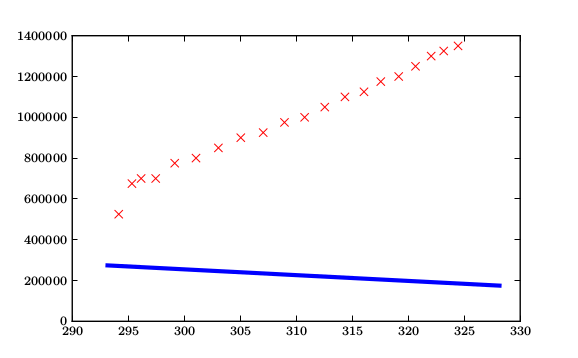
\includegraphics[width=\linewidth-70pt,height=\textheight-70pt,keepaspectratio]{build/Dampdruck.pdf}
 \label{fig:Graph1}
\end{figure}
Daher wird $\ln(Pa)$ gegen die reziproke Temperatur $T_2$ aufgetragen, wie in Abb. \ref{fig:Graph1} dargestellt. Das gesuchte $L$ ist proportional zur Steigung des Graphen.
Mithilfe einer linearen Ausgleichsrechnung der Form $y=Ax+b$ mittels scipy
berechnet sich nun die Steigung. Für $L$ folgt dann:
\begin{equation}
  L = -A\cdot R\text{.}\label{eq:LausA}
\end{equation}
Mit einem $R = \num{8.3144598(48)}$ \cite{R} folgt eine Verdampfungswärme von $L = \SI{1.13(5)e6}{\joule\per\kilo\per\gram}$
Unter Verwendung der bereits bei der Güte verwendeten Wärmekapazitäten und der gleichen
 Menge Wasser sowie dem nun bestimmten $L$ berechnet sich der Massendurchsatz. Dieser ist in Tabelle \ref{tab:tabm} dargestellt.

 \begin{table}
   \centering
   \caption{Der bestimmte Massendurchsatz zu 4 verschiedenen Zeitpunkten.}
   \input{build/tabm.tex}\label{tab:massen}
 \end{table}

\subsection{Bestimmung der Leistung mithilfe des Massendurchsatzes}
Zuletzt wird auch die bestehende Leistung aus den bereits errechneten Daten zu den 4 Zeitpunkten bestimmt.
Dies geschieht mithilfe von Formel \ref{eq:Nmech}. Daher muss zunächst die Temperatur
und Druckabhängige Dichtefunktion bestimmt werden. Diese folgt aus der allgemeinen Gasgleichung:
\begin{equation}
  p\cot V = n\cdot R\cdot T\text{.}
\end{equation}
Durch Umformung ergibt sich:
\begin{equation}
  \rho(p,T) = \frac{p\cdot \rho_0\cdot T_0}{p_0\cdot T}
\end{equation}
Mit einem $\rho_0 = \SI{5.51}{\gram\per\litre}$ \cite{V206} bei einem Normaldruck $p_0 = \SI{1}{\bar}$
und einer Normaltemperatur $T_0 = \SI{273.15}{\kelvin}$ sowie einem $\kappa = 1.44$ \cite{V206} ergeben sich die Leistungen in Tabelle \ref{tab:tabn}.

\begin{table}
  \centering
  \caption{Die bestimmte Leistung zu 4 verschiedenen Zeitpunkten.}
  \input{build/tabn.tex}\label{tab:Leistung}
\end{table}
